\subsection{Construction de l'ensemble stable maximal}\label{mis}
La première étape de l'algorithme consiste en la construction du MIS dont la définition est la suivante et qui possède des propriétés intéressantes pour la suite :
\begin{defn}Soit $G=(V,E)$ un graphe, l'ensemble stable maximal est le plus grand sous-ensemble $S\subseteq V$ tel que le sous-graphe $G[S]$ induit par $S$ ne contient pas d'arêtes.\end{defn}

\begin{lemma}\label{lmmis1}
Dans tout graphe géométrique, la taille de ses ensembles stables maximaux est majorée par $3.8opt+1.2$ où $opt$ est la taille de l'ensemble connexe dominant minimum.
\end{lemma}

\begin{lemma}\label{lmmis2}
Toute paire de sous-ensembles complémentaires du MIS a exactement une distance de deux sauts.
\end{lemma}

\cref{lmmis1} garantit que le ratio de la solution de cet algorithme par rapport à la solution optimale est bien $4.8 + ln5$. La validité de ce lemme dépend beaucoup de nos choix d'implémentation pour les algorithmes de construction MIS. Ces algorithmes étant prévus pour fonctionner de façon distribuée, nos implémentations, non distribuées, ne se comporte donc pas exactement comme ceux-ci.

\cref{lmmis2} est d'une importance majeure pour la validité de la solution. En effet, si une paire de sous-ensembles complémentaires du MIS a une distance inférieure à deux sauts, le MIS sera plus grand que prévu. On risque donc dans ce cas d'obtenir un résultat final plus grand.
À l'inverse, si la distance entre deux sous ensembles complémentaires du MIS est de plus de deux sauts. L'algorithme, essayant de relier ces sous-ensembles du MIS en colorant des nœuds contenant au minimum un voisin dans chacun de ces sous ensembles, ne pourra pas relier ces deux sous-ensembles. L'ensemble obtenu sera constitué d'au moins 2 composantes connexes correspondant aux deux ensembles complémentaires du MIS ayant une distance de plus de deux sauts.

\paragraph{}
Afin de construire un tel MIS qui répond correctement à ces propriété nous nous sommes appuyés une des références \cite{cardei2002connected} cités par les auteurs de l'article. Comme précédemment dit, nous avons dû adapter l'algorithme pour un fonctionnement dans une architecture non distribuée qui faisait passer des messages entre les différents nœuds afin de connaître l'état du réseau. Dans notre cas, nous nous sommes servis d'un système de marquage pour connaître l'avancement de la construction du MIS :
\begin{itemize}
\item \verb?noir? : nœud dominant, appartient au MIS
\item \verb?gris? : nœud dominé, voisin d'un nœud dominant, n'appartient pas au MIS
\item \verb?blanc? : nœud encore non traité par l'algorithme
\item \verb?blanc actif? : état particulier d'un nœud potentiellement prêt à devenir dominant
\end{itemize}

\paragraph{}
Pour illustrer le fonctionnement de notre algorithme basé sur \cite{cardei2002connected} nous allons prendre l'exemple ci-dessous :
\begin{figure}
   	\begin{minipage}[c]{.46\linewidth}
      	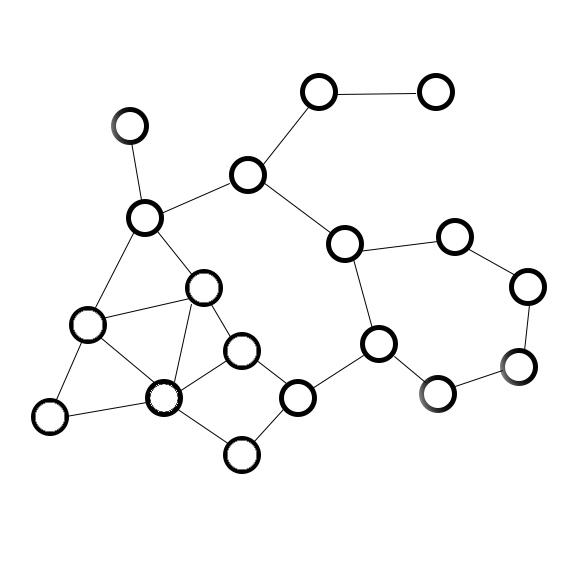
\includegraphics{images/mis1.jpg}
      	\caption{MIS : état initial}
      	\label{mis1}
   	\end{minipage} \hfill
   	\begin{minipage}[c]{.46\linewidth}
      	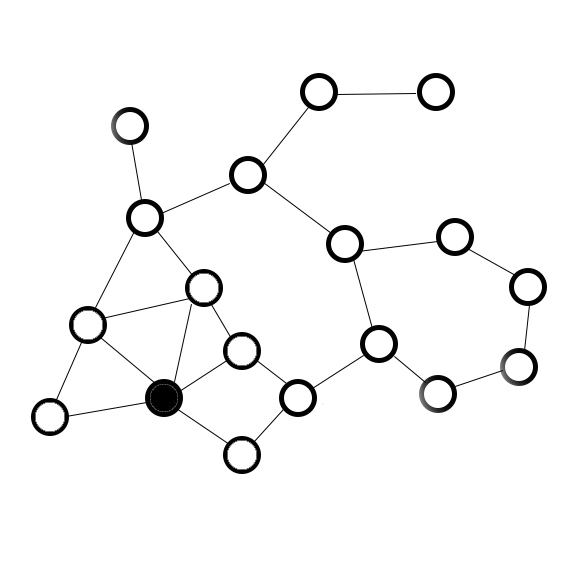
\includegraphics{images/mis2.jpg}
		\caption{MIS : leader}
		\label{mis2}
   	\end{minipage}
\end{figure}

\begin{figure}
   	\begin{minipage}[c]{.46\linewidth}
      	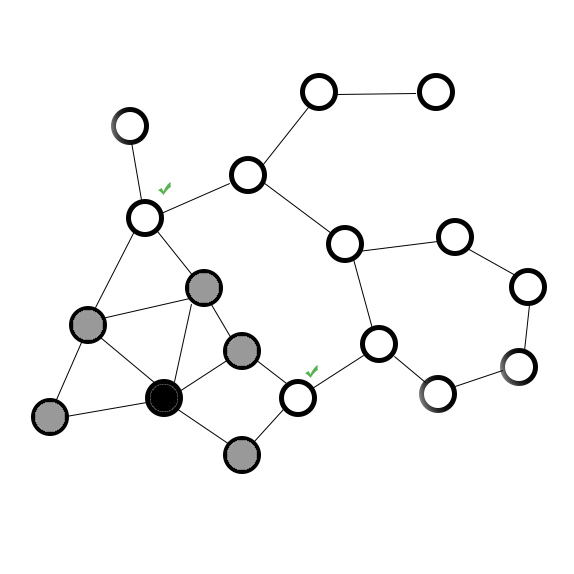
\includegraphics{images/mis3.jpg}
      	\caption{MIS : domination}
      	\label{mis3}
   	\end{minipage} \hfill
   	\begin{minipage}[c]{.46\linewidth}
      	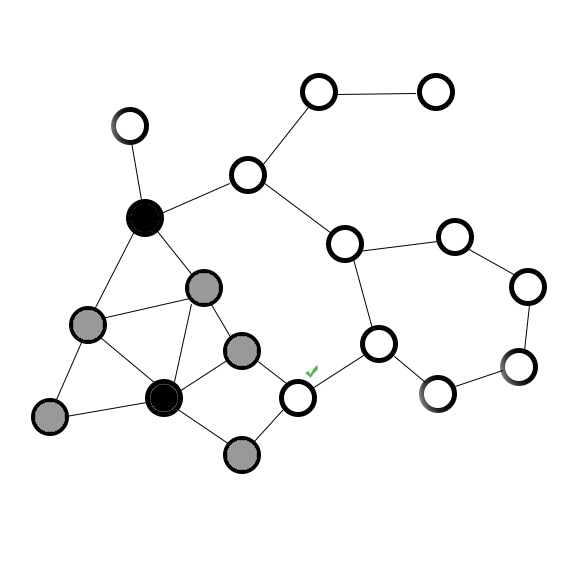
\includegraphics{images/mis4.jpg}
		\caption{MIS : élection}
		\label{mis4}
   	\end{minipage}
\end{figure}

\begin{figure}
   	\begin{minipage}[c]{.46\linewidth}
      	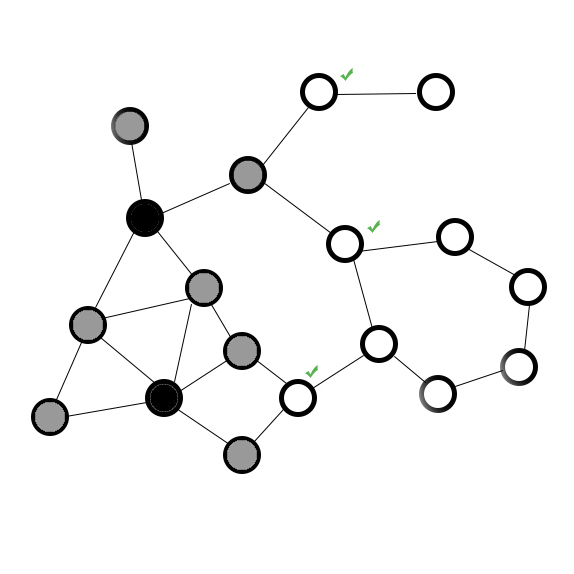
\includegraphics{images/mis5.jpg}
      	\caption{MIS : domination}
      	\label{mis5}
   	\end{minipage} \hfill
   	\begin{minipage}[c]{.46\linewidth}
      	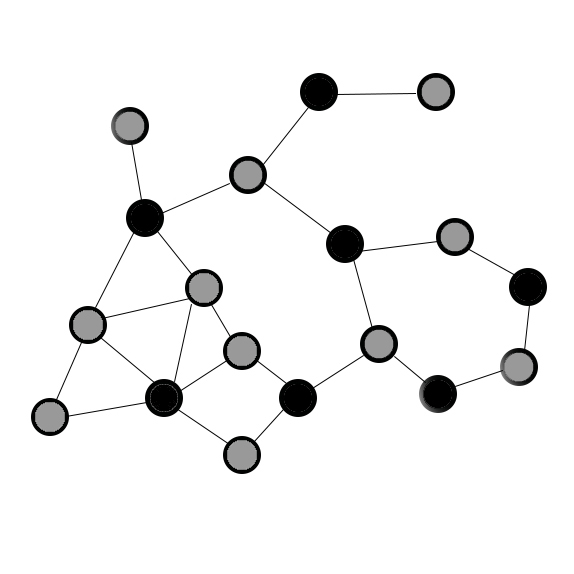
\includegraphics{images/mis6.jpg}
		\caption{MIS : état final}
		\label{mis6}
   	\end{minipage}
\end{figure}

\newpage
L'algorithme commence par choisir un tout premier nœud comme leader, en l'occurrence nous avons fait le choix de prendre le sommet de plus haut degré ce qui semble être pour nous un choix justifié puisque une plus large zone du graphe peut être couvert par ce seul point (figure \ref{mis2}. Ce nœud hôte est ainsi coloré en noir pour marqué son appartenance au MIS et tous ses voisins en gris pour indiquer leur domination par ce dernier.  (figure \ref{mis2}).